\documentclass{beamer}

\usepackage{amsmath}
\usepackage{graphicx}
\usepackage{color}

\title{Obtaining Vibrational Modes of a Clamped Rectangular Membrane Using Finite Element Analysis}
\author{Daniel Geiyer \and Sigitas Rimkus}

\begin{document}
	\begin{frame}
		\titlepage
	\end{frame}
	
	\begin{frame}{Introduction}
		A rectangular membrane can be considered to be a 2D string.
		\begin{columns}
			\begin{column}{0.5\textwidth}
				The displacement $w(x,y,t)$ of the string can be expressed using the wave equation.
				\begin{align*}
					\frac{\partial^2w}{\partial x^2}+\frac{\partial^2w}{\partial y^2}=\frac{1}{c^2}\frac{\partial^2w}{\partial t^2}
				\end{align*}
				The solution is obtained using the technique of separation of variables.
			\end{column}
			\begin{column}{0.5\textwidth}
				\begin{figure}
					\centering
					\resizebox{\textwidth}{!}{\input{membrane.pdf_t}}
					\caption{Membrane in the $x-y$ plane}
				\end{figure}
			\end{column}
		\end{columns}
		The project goal was to find the mode shapes using FEA
	\end{frame}
	
	\begin{frame}{Solution to the Wave Equation}
		The solution consists of a temporal solution and a spatial solution.
		\begin{align*}
			w_{mn}(x,y,t)=\underbrace{\left(A_{mn}\sin\left(\omega_{mn}ct\right)\right)}_\text{Temporal solution}\underbrace{\sin \left(m\pi x\right)\sin \left(n\pi y\right)}_\text{Spatial solution}
		\end{align*}
		Details on the solution components:
		\begin{itemize}
			\item{Temporal solution contains information on how the displacement of the membrane changes over time.}
			\item{The spatial solution contains information about the mode shapes of the membrane.}
		\end{itemize}
	\end{frame}
	
	\begin{frame}{Analytical solution}
		\begin{figure}
			\centering
			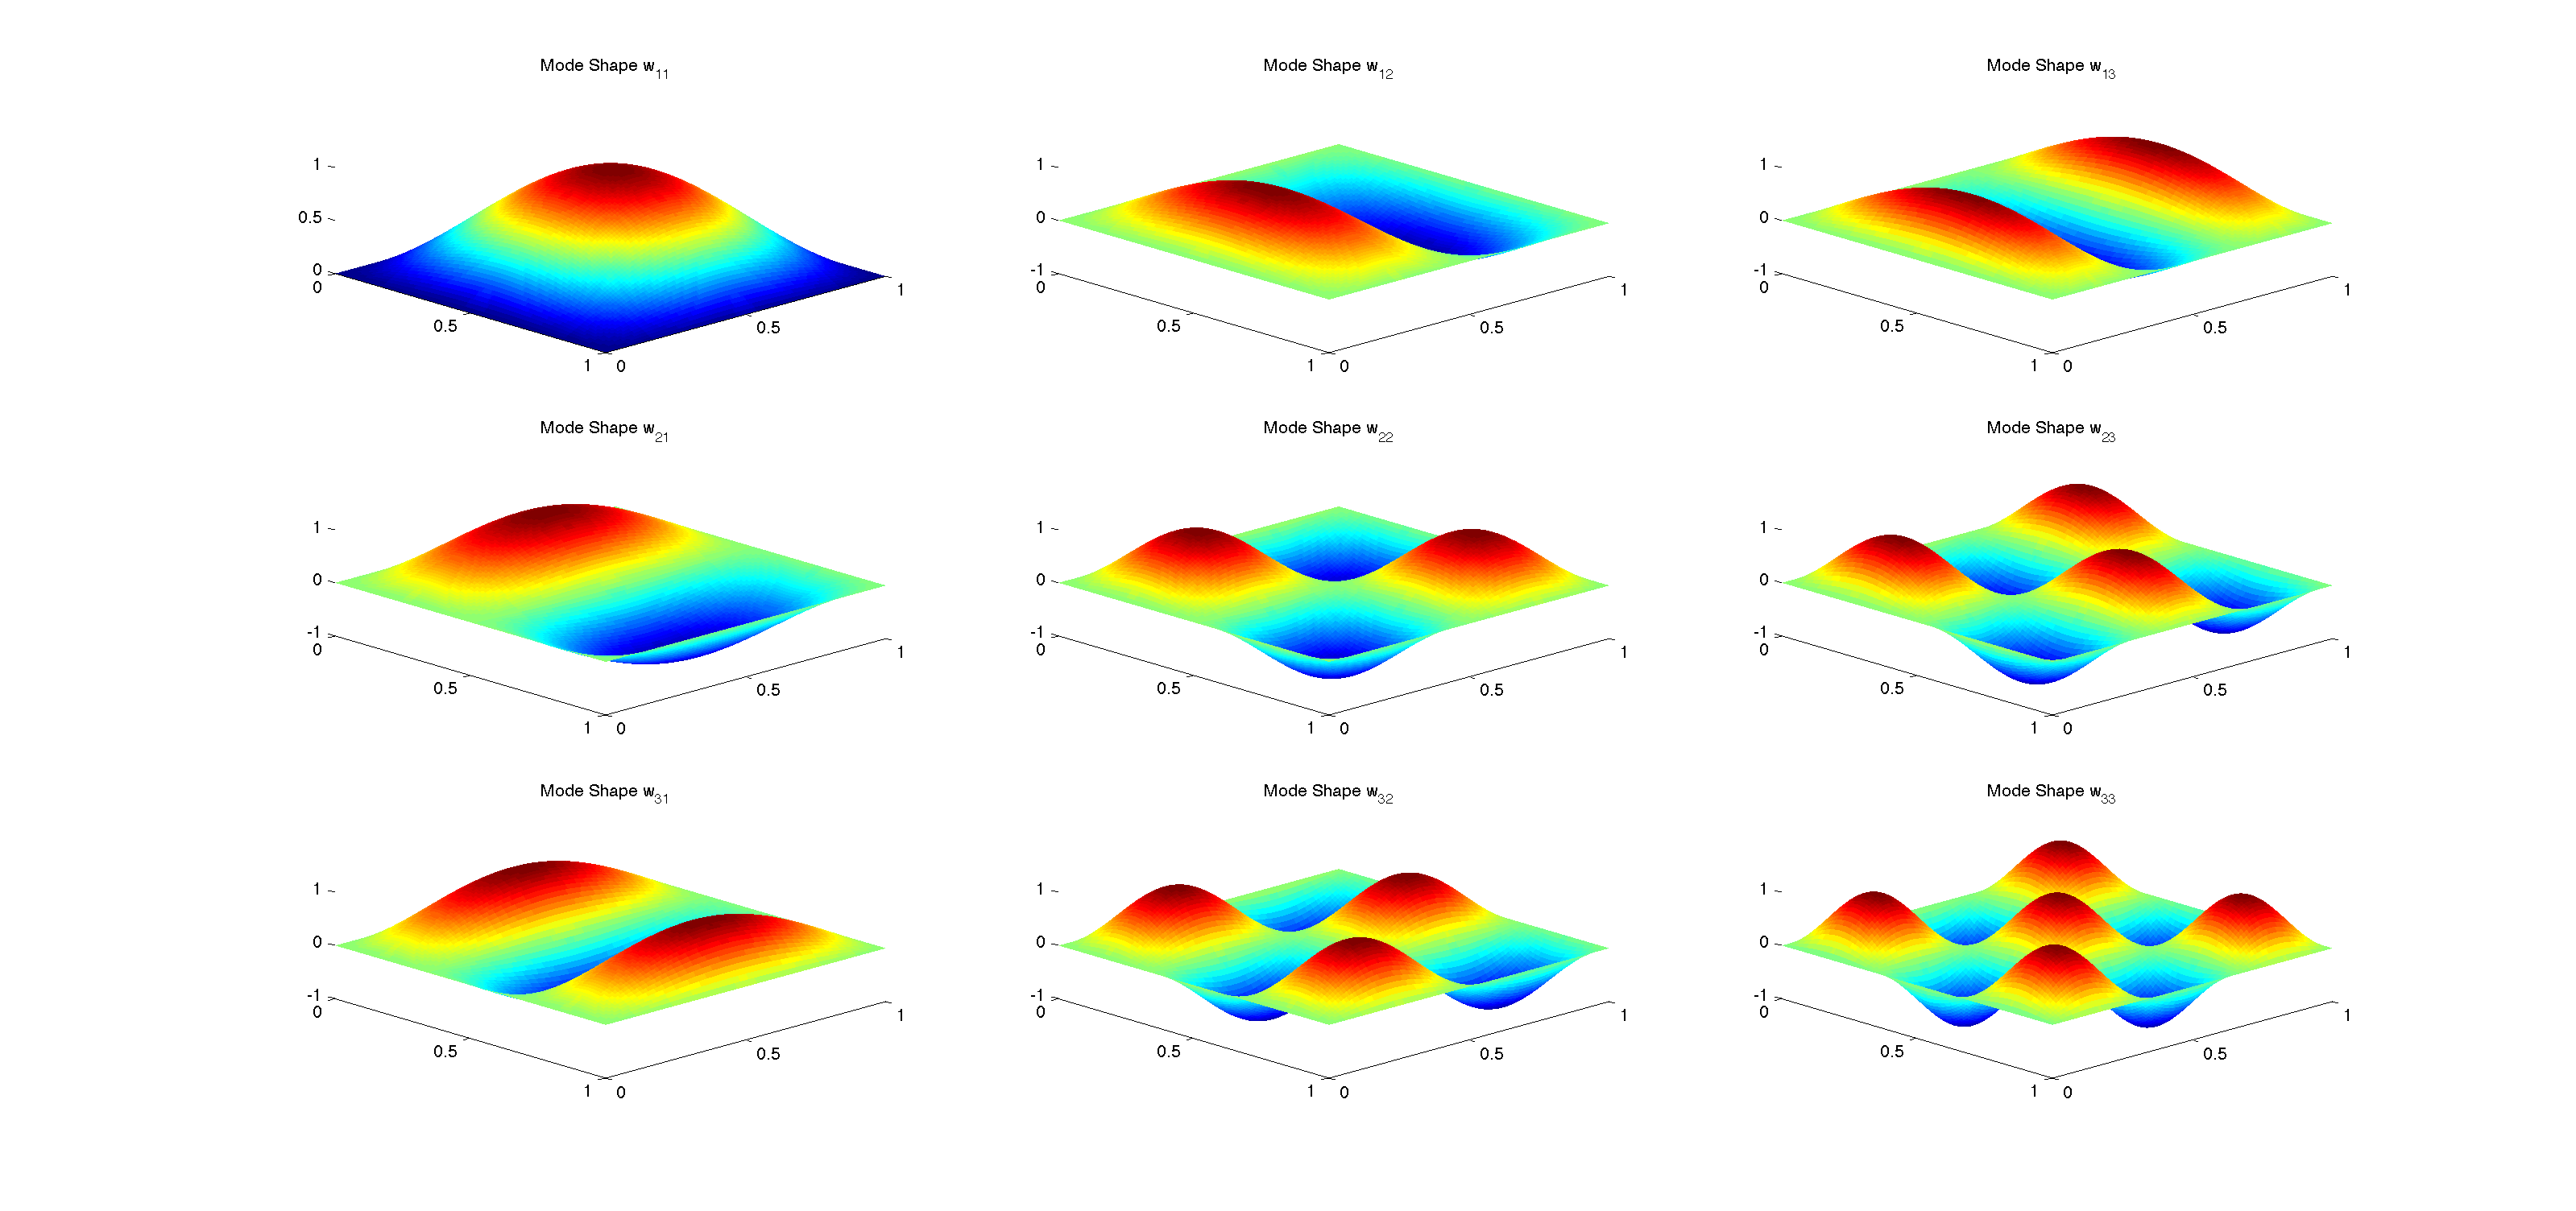
\includegraphics[width=\textwidth]{modes_surf}
		\end{figure}
	\end{frame}

\end{document}